\subsection{Projekt Oversigt} \label{sec:ProjectList}
Dette afsnit indeholder en gennemgang af den grafisk brugergrænseflade, design og implementering af 'Project List' viewet i Rambøll Tilsyn.

\subsubsection{Design}
På Figur \ref{fig:ProjctListSekvens} ses sekvensdiagrammet for 'Project List' viewet til Rambøll Tilsyn.
\begin{figure}[H] % (alternativt [H])
	\centering
	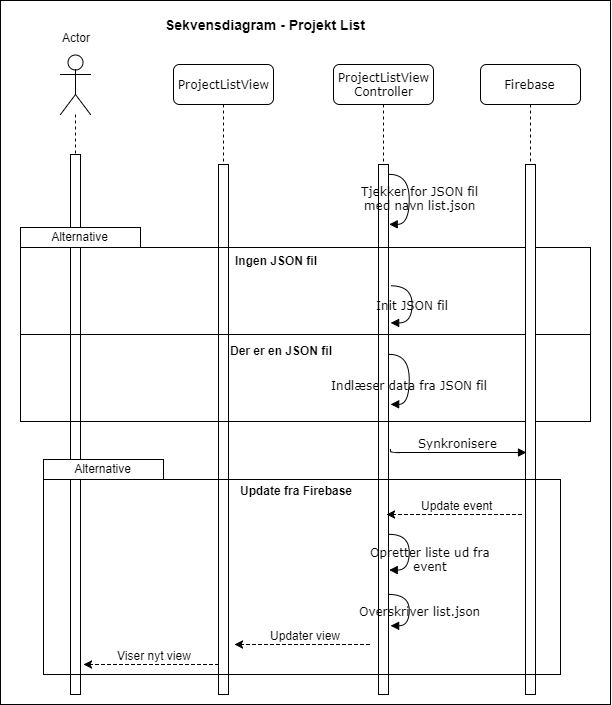
\includegraphics[height=15cm, width=15cm]{../ArkitekturDesign/Design/ProjectList/ProjektListSekvensDiagram}
	\caption{Sekvensdiagram for ProjectList i Rambøll Tilsyn.}
	\label{fig:ProjctListSekvens}
\end{figure}

\clearpage

\subsubsection{Grafisk brugergrænseflade}
I ProjectListViewet er der en oversigt over, hvilke projekter der ligger i databasen, samt mulighed for øverst at tilføje projekt eller tilføj bruger. Se Figur \ref{fig:ProjectListView}
\begin{figure}[H] % (alternativt [H])
	\centering
	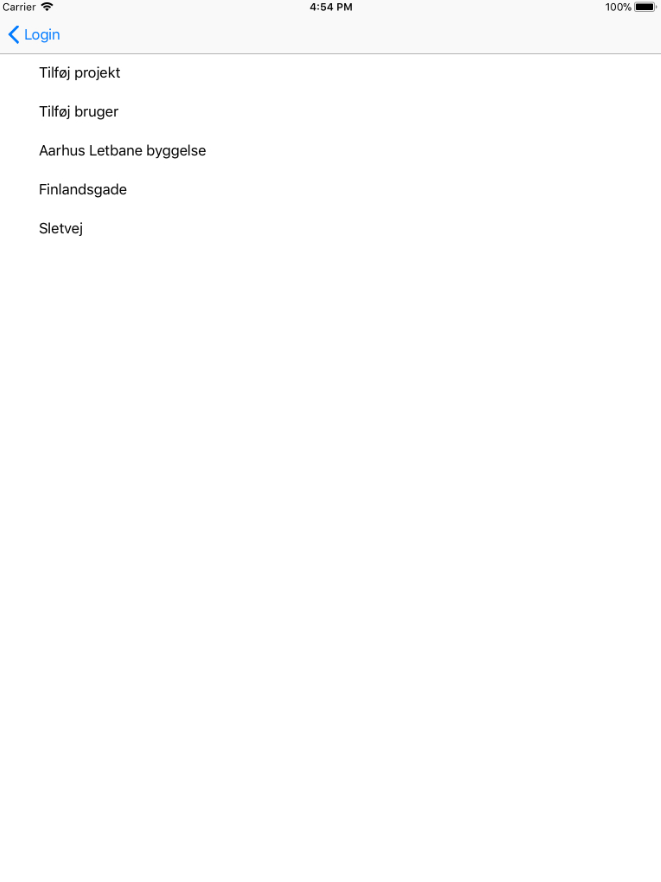
\includegraphics[height=12cm, width=10cm]{../ArkitekturDesign/Design/ProjectList/ProjectList}
	\caption{'Project List' viewet, som det er implementeret i Rambøll Tilsyn.}
	\label{fig:ProjectListView}
\end{figure}

\clearpage

\subsubsection{Implementering}
I dette afsnit vil der blive beskrevet funktionaliteten for de vigtigste funktioner i koden tilhørende 'Project List' viewet.

På Figur \ref{fig:ProjectListViewController}, ses funktionen for ProjectListViewController().
\begin{figure}[H] % (alternativt [H])
	\centering
	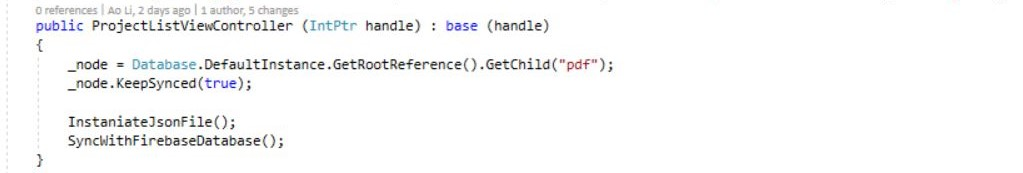
\includegraphics[height=3cm, width=17cm]{../ArkitekturDesign/Design/ProjectList/ProjectListViewController}
	\caption{Kode snip - ProjectListViewController() fra ProjectListViewController.cs}
	\label{fig:ProjectListViewController}
\end{figure}
Det første er, at der hentes en reference node med navn PDF fra Firebase og fortæller at denne node skal holdes synkroniseret, i tilfælde af dataændring. \\
Efterfølgende initialiseres JSON-filen og synkrorinisere efterfølgende med Firebase.

På Figur \ref{fig:JSONFile}, ses funktionen for InstaniateJsonFile().
\begin{figure}[H] % (alternativt [H])
	\centering
	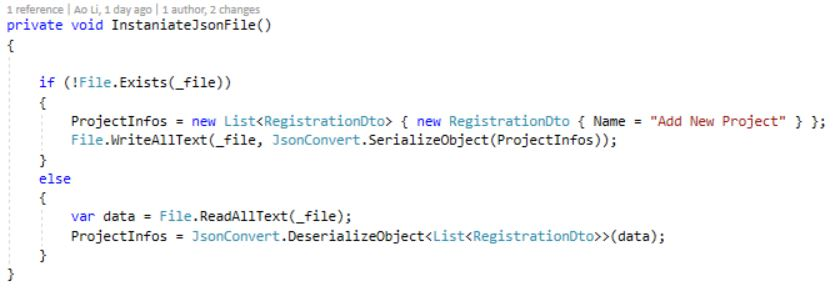
\includegraphics[height=5cm, width=15cm]{../ArkitekturDesign/Design/ProjectList/JSONFile}
	\caption{Kode snip - InstaniateJsonFile() fra ProjectListViewController.cs}
	\label{fig:JSONFile}
\end{figure}
Der oprettes en JSON-fil, hvis der ikke findes en i forvejen. Denne gemmes lokalt.\\
Hvis der findes en JSON-fil, læses data fra filen.

\clearpage

På Figur \ref{fig:SyncWithDB}, ses funktionen for SyncWithFirebaseDatabase().
\begin{figure}[H] % (alternativt [H])
	\centering
	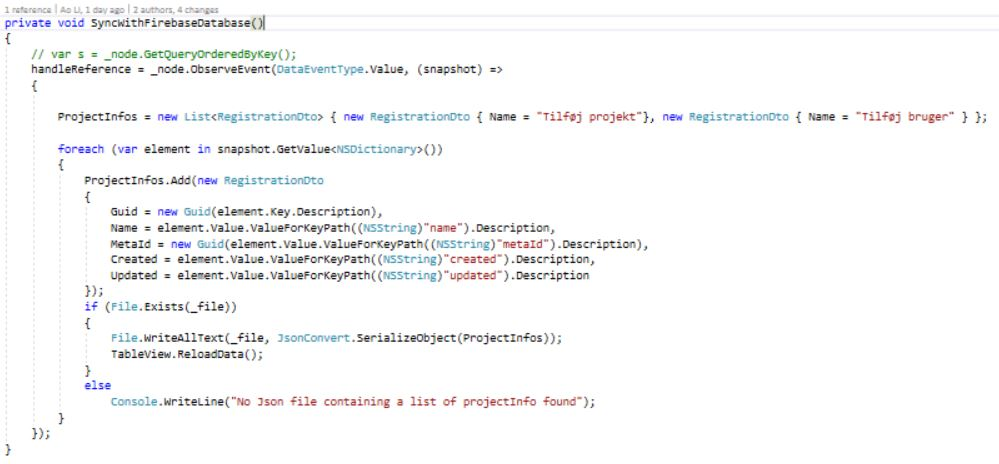
\includegraphics[height=8cm, width=15cm]{../ArkitekturDesign/Design/ProjectList/SyncWithDB}
	\caption{Kode snip - SyncWithFirebaseDatabase() fra ProjectListViewController.cs}
	\label{fig:SyncWithDB}
\end{figure}
Noden, som er oprettet i konstrukteren, som ses på Figur \ref{fig:ProjectListViewController}, den vedhæftes til et event, som kaldes hver gang noden ændres. \\
Når eventet kaldes, læses data fra eventet og gemmer dette i JSON filen. Efterfølgende fortælles controlleren at viewet skal opdateres.

På Figur \ref{fig:ViewDidLoad}, ses funktionen for ViewDidLoad().
\begin{figure}[H] % (alternativt [H])
	\centering
	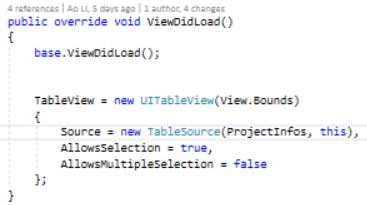
\includegraphics[height=5cm, width=10cm]{../ArkitekturDesign/Design/ProjectList/ViewDidLoad}
	\caption{Kode snip - ViewDidLoad() fra ProjectListViewController.cs}
	\label{fig:ViewDidLoad}
\end{figure}
Her sættes ListViewets source til at være TableSource.

\clearpage

På Figur \ref{fig:TableSource}, ses funktionen for TableSource().
\begin{figure}[H] % (alternativt [H])
	\centering
	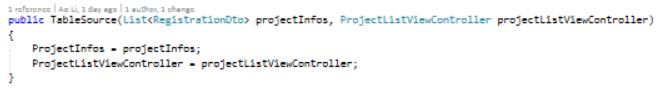
\includegraphics[height=2cm, width=15cm]{../ArkitekturDesign/Design/ProjectList/TableSource}
	\caption{Kode snip - TableSource() fra TableSource.cs}
	\label{fig:TableSource}
\end{figure}
Der initialiseres, hvilke værdier der skal fremvises og der er givet en reference til ProjctListViewControlleren.

På Figur \ref{fig:RowSelection}, ses funktionen for RowSelected().
\begin{figure}[H] % (alternativt [H])
	\centering
	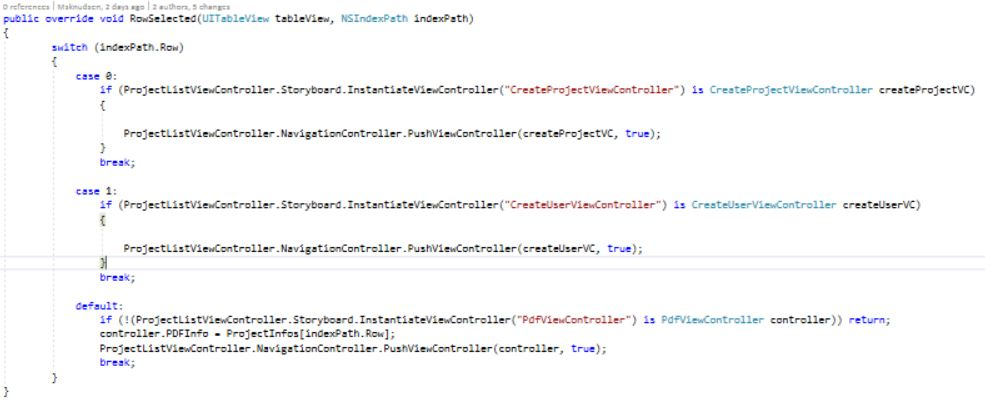
\includegraphics[height=8cm, width=17cm]{../ArkitekturDesign/Design/ProjectList/RowSelection}
	\caption{Kode snip - RowSelected() fra TableSource.cs}
	\label{fig:RowSelection}
\end{figure}
Der er en switch case, case CreateProject giver bruger mulighed for at navigere til 'Opret projekt' siden. Case CreateUser navigere brugeren til 'Opret bruger' siden. \\
Ellers skal den navigere brugeren til 'PDFViewControlleren', for det valgte projekt.

\clearpage
